\chapter{Learning Algorithms}
\label{app:Learning}


\section{Support Vector Machines}
Support Vector Machines (SVMs) are a set of supervised learning methods used for classification, regression, and outliers detection. The basic SVM takes input data and predicts, for each given input, which of two possible classes the input is a part of, making it a non-probabilistic binary linear classifier.


The core idea behind SVM is to find the hyperplane that best divides a dataset into two classes. Features of the input data are used to plot each data item as a point in n-dimensional space (where n is the number of features), with the value of each feature being the value of a particular coordinate. Then, SVM performs classification by finding the hyperplane that best separates the two classes.

\subsection*{Mathematical Formulation}
The decision function of an SVM is defined as:
\[ f(x) = \mathbf{w}^T\mathbf{x} + b \]
where $\mathbf{w}$ is the weight vector, $\mathbf{x}$ is the feature vector, and $b$ is the bias.

The goal of the SVM algorithm is to find the values of $\mathbf{w}$ and $b$ that maximize the margin between the two classes. This is typically done by solving a convex optimization problem.


The optimization problem for finding \(\mathbf{w}\) and \(b\) is formulated as:
\[
\min_{\mathbf{w}, b} \frac{1}{2} \|\mathbf{w}\|^2 + C \sum_{i=1}^{n} \xi_i
\]
Subject to:
\[
y_i (\mathbf{w}^T \mathbf{x_i} + b) \geq 1 - \xi_i, \quad \xi_i \geq 0, \quad i=1,...,n
\]
where \(y_i \in \{-1, 1\}\) are class labels, \(C\) is the regularization parameter, and \(\xi_i\) are slack variables.


The Lagrangian dual problem is given by:
\[
\max_{\alpha} \left[ \sum_{i=1}^{n} \alpha_i - \frac{1}{2} \sum_{i,j=1}^{n} y_i y_j \alpha_i \alpha_j \langle \mathbf{x_i}, \mathbf{x_j} \rangle \right]
\]
Subject to:
\[
\sum_{i=1}^{n} \alpha_i y_i = 0, \quad 0 \leq \alpha_i \leq C, \quad i=1,...,n
\]


After solving the dual problem, \(\mathbf{w}\) and \(b\) are obtained as follows:
\[
\mathbf{w} = \sum_{i=1}^{n} \alpha_i y_i \mathbf{x_i}
\]
\[
b = y_s - \mathbf{w}^T \mathbf{x_s}
\]
for any support vector \(x_s\) with \(0 < \alpha_s < C\).

The decision function can be expressed as:
\[
f(x) = \sum_{i=1}^{n} \alpha_i y_i \langle \mathbf{x}, \mathbf{x_i} \rangle + b
\]

\newpage

\section{Learning Alghoritms}


\subsection*{Deep Deterministic Policy Gradient (DDPG)}

When considering learning, one key concept is interaction with the environment, which provides feedback on actions taken to achieve goals. Reinforcement Learning (RL) is a machine learning technique that utilizes this interaction to identify optimal behavior within an environment. The objective in RL is to determine a policy—a mapping from states to actions—that maximizes the total expected reward, which can be accrued in both terminal and intermediate states. RL involves an agent gaining experience with states, actions, state transitions, and rewards to iteratively refine its behavior towards optimality. Unlike other machine learning paradigms, RL systems are evaluated concurrently with the learning process through trial-and-error, balancing exploration and exploitation.

RL employs a sequential decision process formalized as a Markov Decision Process (MDP), defined by a tuple \( M = \langle S,A,T,R \rangle \):
\begin{itemize}
	\item A finite set of states \( S \).
	\item A finite set of actions \( A \).
	\item A state transition function \( T(s' | s,a) \) giving the probability of transitioning to state \( s' \) when action \( a \) is performed in state \( s \).
	\item A reward function \( R \) indicating the desirability of state-action transitions, which can be simplified to \( R(s,a) \) representing the expected reward for taking action \( a \) in state \( s \).
\end{itemize}

The cumulative reward \( G_t \) obtained from time \( t \) onwards is defined as:

\[ G_t = \sum_{k=t}^{\infty} \gamma^{k-t} R(s_k, a_k) \]

where \( \gamma \) is the discount factor.

Key elements in RL include:
\begin{itemize}
	\item The policy \( \pi \), a mapping from states to actions that determines the system's behavior.
	\item The value function \( V^{\pi}(s) \), representing the expected cumulative reward from state \( s \) under policy \( \pi \):
	
	\[ V^{\pi}(s) = \mathbb{E}_{\pi} [G_t | s_t = s] \]
	
	\item The action-value function \( Q^{\pi}(s,a) \), representing the expected cumulative reward from state \( s \) by taking action \( a \) and then following policy \( \pi \):
	
	\[ Q^{\pi}(s,a) = \mathbb{E}_{\pi} [G_t | s_t = s, a_t = a] \]
\end{itemize}

The Bellman equation for the state-value function \( V^{\pi} \) is:

\[ V^{\pi}(s) = \mathbb{E}_{\pi} [R(s,a) + \gamma V^{\pi}(s') | s_t = s] \]

Dynamic Programming (DP), Monte Carlo (MC), and Temporal Differences (TD) are three main methods to solve MDPs. DP assumes knowledge of transition and reward functions, MC learns from complete episodes, and TD combines elements of both by updating based on the current estimate and sampling.

In scenarios with large state-action spaces, traditional tabular methods become impractical. This is where deep RL, which combines RL with deep neural networks, becomes valuable. The Deep-Q Network (DQN) algorithm was a groundbreaking advancement, achieving superhuman performance in Atari games by approximating Q-values with neural networks. DQN introduced key innovations like experience replay and fixed Q-targets to stabilize learning.

However, DQN is limited to discrete action spaces. To address this, the Deep Deterministic Policy Gradient (DDPG), reported in Figure\tildeAdd\ref{fig:act_crit}, algorithm was developed for continuous action spaces~\cite{sutton2018reinforcement}. DDPG employs an actor-critic architecture with separate networks for the actor and critic:

\begin{itemize}
	\item \textbf{Critic Network:} Approximates the action-value function \( Q_{\phi}(s, a) \). It is trained to minimize the Bellman error using a mean squared error loss:
	
	\[
	L(\phi) = \mathbb{E}\left[\left(Q_{\phi}(s_t, a_t) - \left(r_{t+1} + \gamma \max_{a_{t+1}} Q_{\phi'}(s_{t+1}, a_{t+1})\right)\right)^2\right]
	\]
	
	Here, \( \phi \) represents the parameters of the critic network, and \( \phi' \) are the parameters of a target critic network, which are periodically updated to provide stable targets for learning.
	
	\item \textbf{Actor Network:} Represents the policy \( \pi_{\theta}(s) \), mapping states to actions. It is trained to maximize the expected Q-value, using the critic's estimates to guide the policy improvement:
	
	\[
	\max_{\theta} \mathbb{E}_{s \sim \mathcal{D}}\left[Q_{\phi}(s, \pi_{\theta}(s))\right]
	\]
	
	Here, \( \theta \) represents the parameters of the actor network.
\end{itemize}

\begin{figure}
	\centering
	\tikzset{every picture/.style={line width=0.75pt}} %set default line width to 0.75pt        
	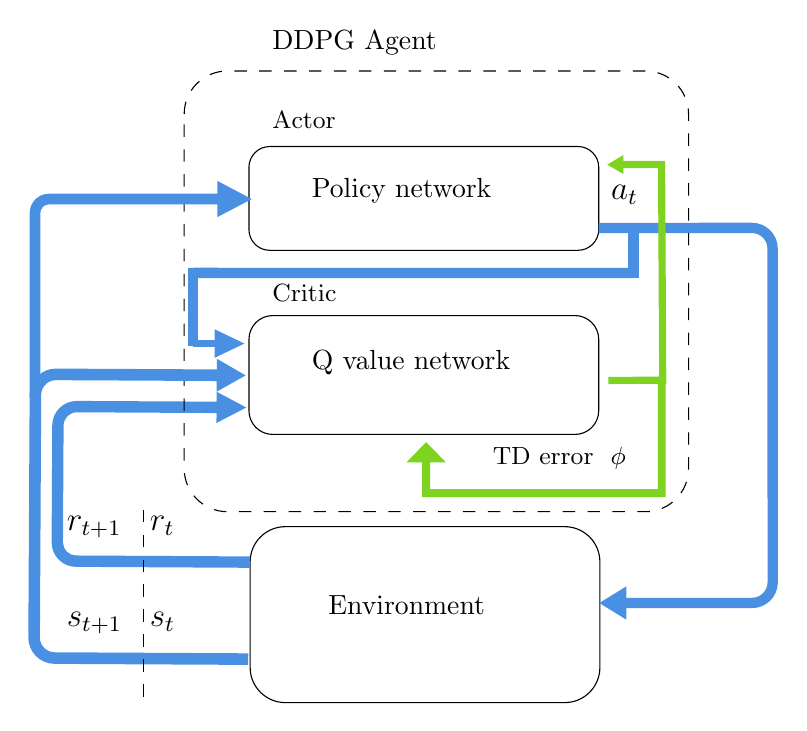
\begin{tikzpicture}[x=0.75pt,y=0.75pt,yscale=-1,xscale=1]
		%uncomment if require: \path (0,384); %set diagram left start at 0, and has height of 384
		
		%Rounded Rect [id:dp7665134511880258] 
		\draw   (253,93) .. controls (253,87.48) and (257.48,83) .. (263,83) -- (411.52,83) .. controls (417.04,83) and (421.52,87.48) .. (421.52,93) -- (421.52,123) .. controls (421.52,128.52) and (417.04,133) .. (411.52,133) -- (263,133) .. controls (257.48,133) and (253,128.52) .. (253,123) -- cycle ;
		%Rounded Rect [id:dp8334704830076491] 
		\draw   (253,175.89) .. controls (253,169.57) and (258.13,164.44) .. (264.46,164.44) -- (410.06,164.44) .. controls (416.39,164.44) and (421.52,169.57) .. (421.52,175.89) -- (421.52,210.26) .. controls (421.52,216.58) and (416.39,221.71) .. (410.06,221.71) -- (264.46,221.71) .. controls (258.13,221.71) and (253,216.58) .. (253,210.26) -- cycle ;
		%Rounded Rect [id:dp7924498191432374] 
		\draw   (253.58,283.1) .. controls (253.58,273.73) and (261.18,266.14) .. (270.54,266.14) -- (405.13,266.14) .. controls (414.49,266.14) and (422.08,273.73) .. (422.08,283.1) -- (422.08,333.97) .. controls (422.08,343.33) and (414.49,350.92) .. (405.13,350.92) -- (270.54,350.92) .. controls (261.18,350.92) and (253.58,343.33) .. (253.58,333.97) -- cycle ;
		%U Turn Arrow [id:dp5830248631009427] 
		\draw  [draw opacity=0][fill={rgb, 255:red, 74; green, 144; blue, 226 }  ,fill opacity=1 ] (421.53,119.74) -- (495.32,119.71) .. controls (502.2,119.71) and (507.78,125.29) .. (507.78,132.16) -- (507.83,292.94) .. controls (507.84,299.82) and (502.26,305.4) .. (495.39,305.4) -- (434.81,305.42) -- (434.81,310.94) -- (421.8,302.93) -- (434.81,294.92) -- (434.81,300.43) -- (495.38,300.41) .. controls (499.51,300.41) and (502.85,297.07) .. (502.85,292.94) -- (502.79,132.16) .. controls (502.79,128.04) and (499.45,124.7) .. (495.32,124.7) -- (421.53,124.73) -- cycle ;
		%U Turn Arrow [id:dp7331227116017869] 
		\draw  [draw opacity=0][fill={rgb, 255:red, 126; green, 211; blue, 33 }  ,fill opacity=1 ] (426.2,197.43) -- (453.9,197.28) .. controls (454.01,197.28) and (454.09,197.2) .. (454.09,197.09) -- (453.51,90.05) .. controls (453.51,89.94) and (453.43,89.86) .. (453.32,89.86) -- (433.36,89.96) -- (433.34,87.14) -- (425.63,91.73) -- (433.39,96.24) -- (433.38,93.42) -- (450.08,93.32) .. controls (450.08,93.32) and (450.08,93.32) .. (450.08,93.32) -- (450.62,193.85) .. controls (450.62,193.85) and (450.62,193.85) .. (450.62,193.85) -- (426.19,193.98) -- cycle ;
		%U Turn Arrow [id:dp9250538511454254] 
		\draw  [draw opacity=0][fill={rgb, 255:red, 126; green, 211; blue, 33 }  ,fill opacity=1 ] (453.8,193.85) -- (453.8,251.92) .. controls (453.8,251.92) and (453.8,251.92) .. (453.8,251.92) -- (336.47,251.92) .. controls (336.47,251.92) and (336.47,251.92) .. (336.47,251.92) -- (336.47,235.23) -- (328.8,235.23) -- (338.38,225.42) -- (347.96,235.23) -- (340.29,235.23) -- (340.29,248.1) .. controls (340.29,248.1) and (340.29,248.1) .. (340.29,248.1) -- (449.98,248.1) .. controls (449.98,248.1) and (449.98,248.1) .. (449.98,248.1) -- (449.98,193.85) -- cycle ;
		%U Turn Arrow [id:dp7567739250277439] 
		\draw  [draw opacity=0][fill={rgb, 255:red, 74; green, 144; blue, 226 }  ,fill opacity=1 ] (253.55,285.97) -- (169.68,285.51) .. controls (163.15,285.48) and (157.88,280.15) .. (157.92,273.62) -- (158.22,217.33) .. controls (158.26,210.79) and (163.58,205.52) .. (170.12,205.56) -- (237.41,205.92) -- (237.44,201.14) -- (251.73,208.74) -- (237.35,216.19) -- (237.38,211.41) -- (170.09,211.04) .. controls (166.58,211.02) and (163.72,213.85) .. (163.7,217.36) -- (163.4,273.65) .. controls (163.38,277.15) and (166.21,280.01) .. (169.71,280.03) -- (253.58,280.48) -- cycle ;
		%Rounded Rect [id:dp24819800426709504] 
		\draw  [dash pattern={on 4.5pt off 4.5pt}] (221.8,67.37) .. controls (221.8,55.9) and (231.1,46.6) .. (242.57,46.6) -- (444.03,46.6) .. controls (455.5,46.6) and (464.8,55.9) .. (464.8,67.37) -- (464.8,238.15) .. controls (464.8,249.63) and (455.5,258.92) .. (444.03,258.92) -- (242.57,258.92) .. controls (231.1,258.92) and (221.8,249.63) .. (221.8,238.15) -- cycle ;
		%U Turn Arrow [id:dp7033235171039725] 
		\draw  [draw opacity=0][fill={rgb, 255:red, 74; green, 144; blue, 226 }  ,fill opacity=1 ] (252.64,332.75) -- (159.32,332.25) .. controls (152.31,332.21) and (146.66,326.5) .. (146.7,319.49) -- (147.33,202.6) .. controls (147.37,195.59) and (153.08,189.94) .. (160.09,189.98) -- (237.49,190.39) -- (237.52,185.24) -- (251.39,193.26) -- (237.44,201.14) -- (237.46,195.98) -- (160.06,195.56) .. controls (156.14,195.54) and (152.94,198.7) .. (152.92,202.63) -- (152.29,319.52) .. controls (152.27,323.44) and (155.43,326.64) .. (159.35,326.66) -- (252.67,327.16) -- cycle ;
		%Bend Arrow [id:dp6257279516107521] 
		\draw  [draw opacity=0][fill={rgb, 255:red, 74; green, 144; blue, 226 }  ,fill opacity=1 ] (147.36,203.6) -- (147.36,115.02) .. controls (147.36,109.89) and (151.52,105.72) .. (156.66,105.72) -- (237.76,105.72) -- (237.76,99.57) -- (254.36,108.29) -- (237.76,117.01) -- (237.76,110.86) -- (156.66,110.86) .. controls (154.36,110.86) and (152.5,112.72) .. (152.5,115.02) -- (152.5,203.6) -- cycle ;
		%Straight Lines [id:da09269833954668538] 
		\draw  [dash pattern={on 4.5pt off 4.5pt}]  (202,348) -- (202,255.72) ;
		%Straight Lines [id:da4265551789273936] 
		\draw [color={rgb, 255:red, 74; green, 144; blue, 226 }  ,draw opacity=1 ][line width=3.75]    (439.3,143.92) -- (226,143.9) ;
		%Straight Lines [id:da03151350707279965] 
		\draw [color={rgb, 255:red, 74; green, 144; blue, 226 }  ,draw opacity=1 ][line width=3.75]    (226,179) -- (226,141.5) ;
		%Straight Lines [id:da8116483898702895] 
		\draw [color={rgb, 255:red, 74; green, 144; blue, 226 }  ,draw opacity=1 ][line width=3.75]    (438.3,146.2) -- (438.3,122.3) ;
		%Straight Lines [id:da1508384624951593] 
		\draw [color={rgb, 255:red, 74; green, 144; blue, 226 }  ,draw opacity=1 ][line width=2.25]    (245.8,177.92) -- (226,177.92) ;
		\draw [shift={(250.8,177.92)}, rotate = 180] [fill={rgb, 255:red, 74; green, 144; blue, 226 }  ,fill opacity=1 ][line width=0.08]  [draw opacity=0] (14.29,-6.86) -- (0,0) -- (14.29,6.86) -- cycle    ;
		
		% Text Node
		\draw (282,180) node [anchor=north west][inner sep=0.75pt]   [align=left] {Q value network};
		% Text Node
		\draw (282,97) node [anchor=north west][inner sep=0.75pt]   [align=left] {Policy network};
		% Text Node
		\draw (290,298) node [anchor=north west][inner sep=0.75pt]   [align=left] {Environment};
		% Text Node
		\draw (204,306) node [anchor=north west][inner sep=0.75pt]  [font=\large] [align=left] {$\displaystyle s_{t}$};
		% Text Node
		\draw (426.24,100.2) node [anchor=north west][inner sep=0.75pt]  [font=\large] [align=left] {$\displaystyle a_{t}$};
		% Text Node
		\draw (369.2,226.43) node [anchor=north west][inner sep=0.75pt]  [font=\small] [align=left] {TD error \ $\displaystyle \phi $};
		% Text Node
		\draw (263,65) node [anchor=north west][inner sep=0.75pt]  [font=\normalsize] [align=left] {{\small Actor}};
		% Text Node
		\draw (263,148) node [anchor=north west][inner sep=0.75pt]  [font=\small] [align=left] {Critic};
		% Text Node
		\draw (164,260) node [anchor=north west][inner sep=0.75pt]  [font=\large] [align=left] {$\displaystyle r_{t+1}$};
		% Text Node
		\draw (204,260) node [anchor=north west][inner sep=0.75pt]  [font=\large] [align=left] {$\displaystyle r_{t}$};
		% Text Node
		\draw (164,306) node [anchor=north west][inner sep=0.75pt]  [font=\large] [align=left] {$\displaystyle s_{t+1}$};
		% Text Node
		\draw (263,26) node [anchor=north west][inner sep=0.75pt]   [align=left] {DDPG Agent};
	\end{tikzpicture}
	\caption{Actor-Critic architecture: the actor produces an action given the current state of the environment, and the critic produces a temporal difference (TD) error signal given the state, the action, and the reward.}
	\label{fig:act_crit}
\end{figure}

To improve stability and efficiency, DDPG employs techniques like experience replay and target networks:
\begin{itemize}
	\item \textbf{Experience Replay:} The agent's experiences are stored in a replay buffer \( \mathcal{D} \), allowing the networks to be trained on random mini-batches of experiences. This breaks the temporal correlation between consecutive experiences and leads to more stable learning.
	\item \textbf{Target Networks:} Separate, slowly-updated target networks for both the actor and critic provide stable targets for the Q-value updates, reducing oscillations and divergence during training.
\end{itemize}

In summary, RL is a powerful framework for learning optimal policies through environmental interaction. The combination of RL with deep learning techniques like DDPG enables effective handling of complex, continuous action spaces, making it a versatile and robust approach for a wide range of applications.
When thinking about learning, one concept that immediately springs to mind is the notion of learning through interaction with the environment. This interaction provides us with insights into the effects of our actions, which can then be used to achieve goals. Reinforcement Learning (RL) is a machine learning technique that uses interactions to identify optimal behavior within an environment. In RL, the goal is to identify a policy—mapping states to actions—that maximizes the total expected reward. Rewards can accrue in both terminal and intermediate states. The agent seeks to gain valuable experience with states, actions, state transitions, and rewards to iteratively refine its behavior towards optimality. Unlike other machine learning paradigms, the evaluation of RL systems unfolds concurrently with the learning process. RL operates through a trial-and-error mechanism, navigating through delayed rewards while striking a balance between exploration and exploitation. More details on the DDPG algorithm can be found in \cite{DDPG}.
